\documentclass{article}
\usepackage{graphicx}
\usepackage[margin=1.5cm]{geometry}
\usepackage{amsmath}

\begin{document}
\twocolumn

\title{Wednesday Warm Up: Unit 6, 7: Momentum Conservation and Statics}
\author{Prof. Jordan C. Hanson}

\maketitle

\section{Memory Bank}

\begin{itemize}
\item $\vec{s} = \vec{\theta} \times \vec{r}$
\item $\vec{v} = \vec{\omega} \times \vec{r}$
\item $F_{\rm C} = mr\omega^2$
\item $\hat{i} \times \hat{j} = \hat{k}$, $\hat{k} \times \hat{i} = \hat{j}$, $\hat{j} \times \hat{k} = \hat{i}$
\item $\hat{i} \times \hat{i} = 0$, $\hat{j} \times \hat{j} = 0$, $\hat{k} \times \hat{k} = 0$
\item $\vec{\tau} = \vec{r} \times \vec{F}$ ... The relationship between \textit{torque}, $\vec{\tau}$, the \textit{moment arm}, $\vec{r}$, and the \textit{force}, $\vec{F}$.
\end{itemize}

\begin{figure}[ht]
\centering
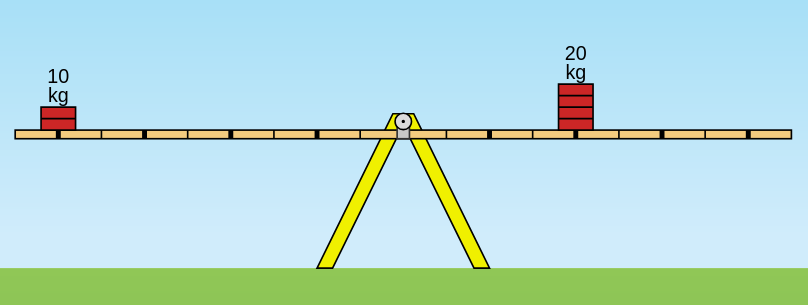
\includegraphics[width=0.45\textwidth]{figures/brick.png}
\caption{\label{fig:1} A balance between bricks of different masses.}
\end{figure}

\section{Two-Dimensional Momentum and Energy Conservation}

\begin{enumerate}
\item Ernest Rutherford (the first New Zealander awarded the Nobel Prize in Chemistry) demonstrated that nuclei were very small and dense by scattering helium-4 nuclei gold-197 nuclei.  The energy of the incoming helium nucleus was $8.00\times10^{-13}$ J, and the masses of the helium and gold nuclei were $6.68\times 10^{-27}$ kg and $3.29\times 10^{-25}$ kg, respectively (the mass ratio is 4 to 197). (a) If a helium nucleus scatters to an angle of 120 degrees during an elastic collision with a gold nucleus, calculate the helium nucleus's final speed and the final velocity (magnitude and direction) of the gold nucleus. (b) What is the final kinetic energy of the helium nucleus? \\ \vspace{5cm}
\end{enumerate}

\section{Fixed Axis Rotation, and Torque}

\begin{enumerate}
\item Suppose a jet fighter complex a 180 degree turn in 15 seconds, with a turn radius of 1500 m. (a) What is the tangential velocity? (b) What is $\omega$? (c) If the jet fighter weighs 19,500 kg, what is $F_{\rm C}$?  \\ \vspace{2cm}
\item Suppose a bolt needs to be unstuck from a flat bulkhead.  Let the bolt be centered at the origin, and let the xy-plane represent the bulkhead.  We must twist it \textit{counterclockwise} to loosen it.  (a) Suppose we have a wrench with length $\vec{r} = 5\hat{i} + 5\hat{j}$ cm attached to the bolt.  If we push on the end of the wrench with $\vec{F} = -10\hat{i}+10\hat{j}$ N of force, what is the \textit{torque} we generate? (b) Why, physically, does the torque vector have the direction we find? (c) List two ways to generate more torque. (d) Sketch $\vec{r}$, $\vec{F}$, and $\vec{\tau}$ below. \\ \vspace{4cm}
\item Consider the balanced system in Fig. \ref{fig:1} (top).  Calculate the net torque due to the masses, assuming a unit of distance along the balance. \\ \vspace{2cm}
\end{enumerate}

\end{document}
